
\chapter{Empirical solar wind model for the inner heliosphere}
\label{chap:empirical_solar_wind_model_for_the_inner_heliosphere}

% introduction
The analyses in the previous chapter are focused on the solar wind's influence on the magnetosphere -- this chapter changes the main focus to the solar wind upstream of the magnetosphere, in a first step down to a solar distance of \SI{0.3}{\au} and then even further down to the region around \SI{10}{\Rs}, close to the solar wind's origin near the Sun. The solar wind's evolution on its way from the near-Sun region to \SI{1}{\au} is modeled with the goal of predicting the solar wind environment for the upcoming Parker Solar Probe (PSP) mission.\\

context of motivation in thesis and paper introduction and context of results in thesis\\

%COFI -- chapter outline and flow integration
This chapter is constructed as follows: first the PSP mission and its scientific goals are described, then I introduce the analyses done in the publication \citet{Venzmer2018}, which constitutes the major part of this chapter. Further, an alternative magnetic field model is derived, which changes the solar distance dependency from the power law in our article to support a Parker magnetic field geometry. Finally, an outlook is given, suggesting different effects that are to be analyzed and quantified further, and could be implemented into the solar wind model.


\section{Parker Solar Probe mission}
Remote observations of the Sun and its corona revealed a wealth of structures and dynamical processes. Over time, most underlying physical mechanisms were identified and the observed features were integrated into a comprehensive picture of the Sun. However, key questions remain unanswered \citep{McComas2007}: It is still unknown how the corona is so much hotter than the chromosphere beneath \citep{Klimchuk2006} and the exact processes involved in the acceleration of the solar wind are not fully understood \citep{Hollweg1985,Cranmer2017}.

Up to now coronal heating and solar wind acceleration remain the open problems that drive the motivation to directly probe the near-Sun environment \citep{McComas2007,Fox2015}. The mission concept of a solar probe taking in-situ measurements from the corona dates back to 1958 when NASA was founded \citep{McComas200807}. The closest solar wind in-situ measurements made so far were done by the two Helios probes, see also \autoref{sec:helios_probes}. Helios~1 was launched in 1974 and reached a perihelion distance of \SI{0.31}{\au} (\SI{67}{\Rs}) and Helios~2 was launched in 1976 and reached a perihelion distance of \SI{0.29}{\au} (\SI{62}{\Rs}) \citep{Rosenbauer1977}. Yet, the solar wind acceleration region is predicted to extend up to the Alfvénic critical surface which lies at solar distances between \SIrange{15}{30}{\Rs} \citep{Katsikas2010,Goelzer2014}. Thus, the Helios spacecraft were well bejond the region where the magic happens.

The Parker Solar Probe (PSP) mission (renamed in 2017 from Solar Probe Plus) is designed to finally address these major questions about the solar corona, in that it will dive into this near-Sun region. The prime goals of the PSP mission as stated by \citet{Fox2015} are: ``Trace the flow of energy that heats and accelerates the solar corona and solar wind; Determine the structure and dynamics of the plasma and magnetic fields at the sources of the solar wind; and Explore mechanisms that accelerate and transport energetic particles.''
These goals seem achievable due to recent developments in technology and engineering that allow PSP to approach the Sun down to a closest distance of \SI{9.86}{\Rs} (\SI{0.046}{\au}) from the center of the Sun. PSP launched on 11~August 2018 and utilizes seven Venus gravity assists over nearly seven years throughout its mission in order to lower its orbit around the Sun, see the planned trajectory in \autoref{fig:PSP_MissionDesign2_negative}.
\begin{figure}
	\fcapside[\FBwidth]{
		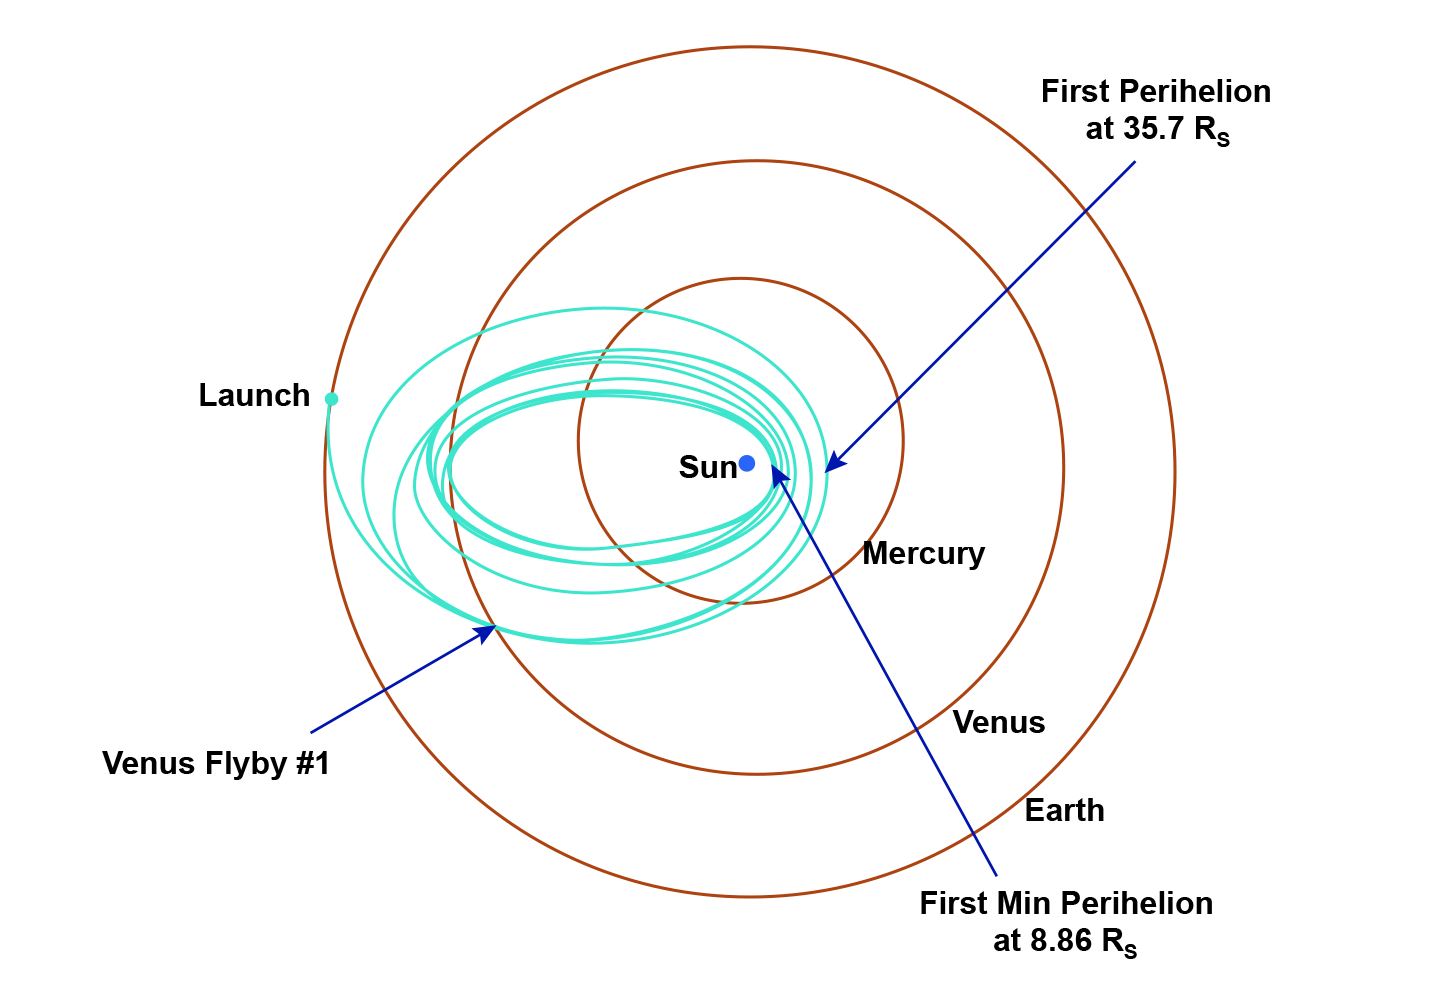
\includegraphics[width=0.6\textwidth]{figures_of_others/images/PSP_MissionDesign2_negative.png}
	}{
		\caption[\lofimage{figures_of_others/images/PSP_MissionDesign2_negative.png}]
		{Trajectory design of the PSP mission in the inner solar system with the positions of the launch, the first Venus flyby, the first perihelion, and the first closest perihelion. Credit: \href{http://parkersolarprobe.jhuapl.edu/The-Mission/index.php}{NASA/Johns Hopkins APL}, 2018 (the colors are inverted).}
		\label{fig:PSP_MissionDesign2_negative}
	}
\end{figure}

The proximity to the Sun during the perihelia requires a sunward heat shield as well as a big heat radiator system behind to protect the instruments on the spacecraft's body -- both are shown in the illustration of PSP flying near the Sun in \autoref{fig:SPP_ObservingSun2}.
\begin{figure}[htb]
	\begin{floatrow}
		\ffigbox{
			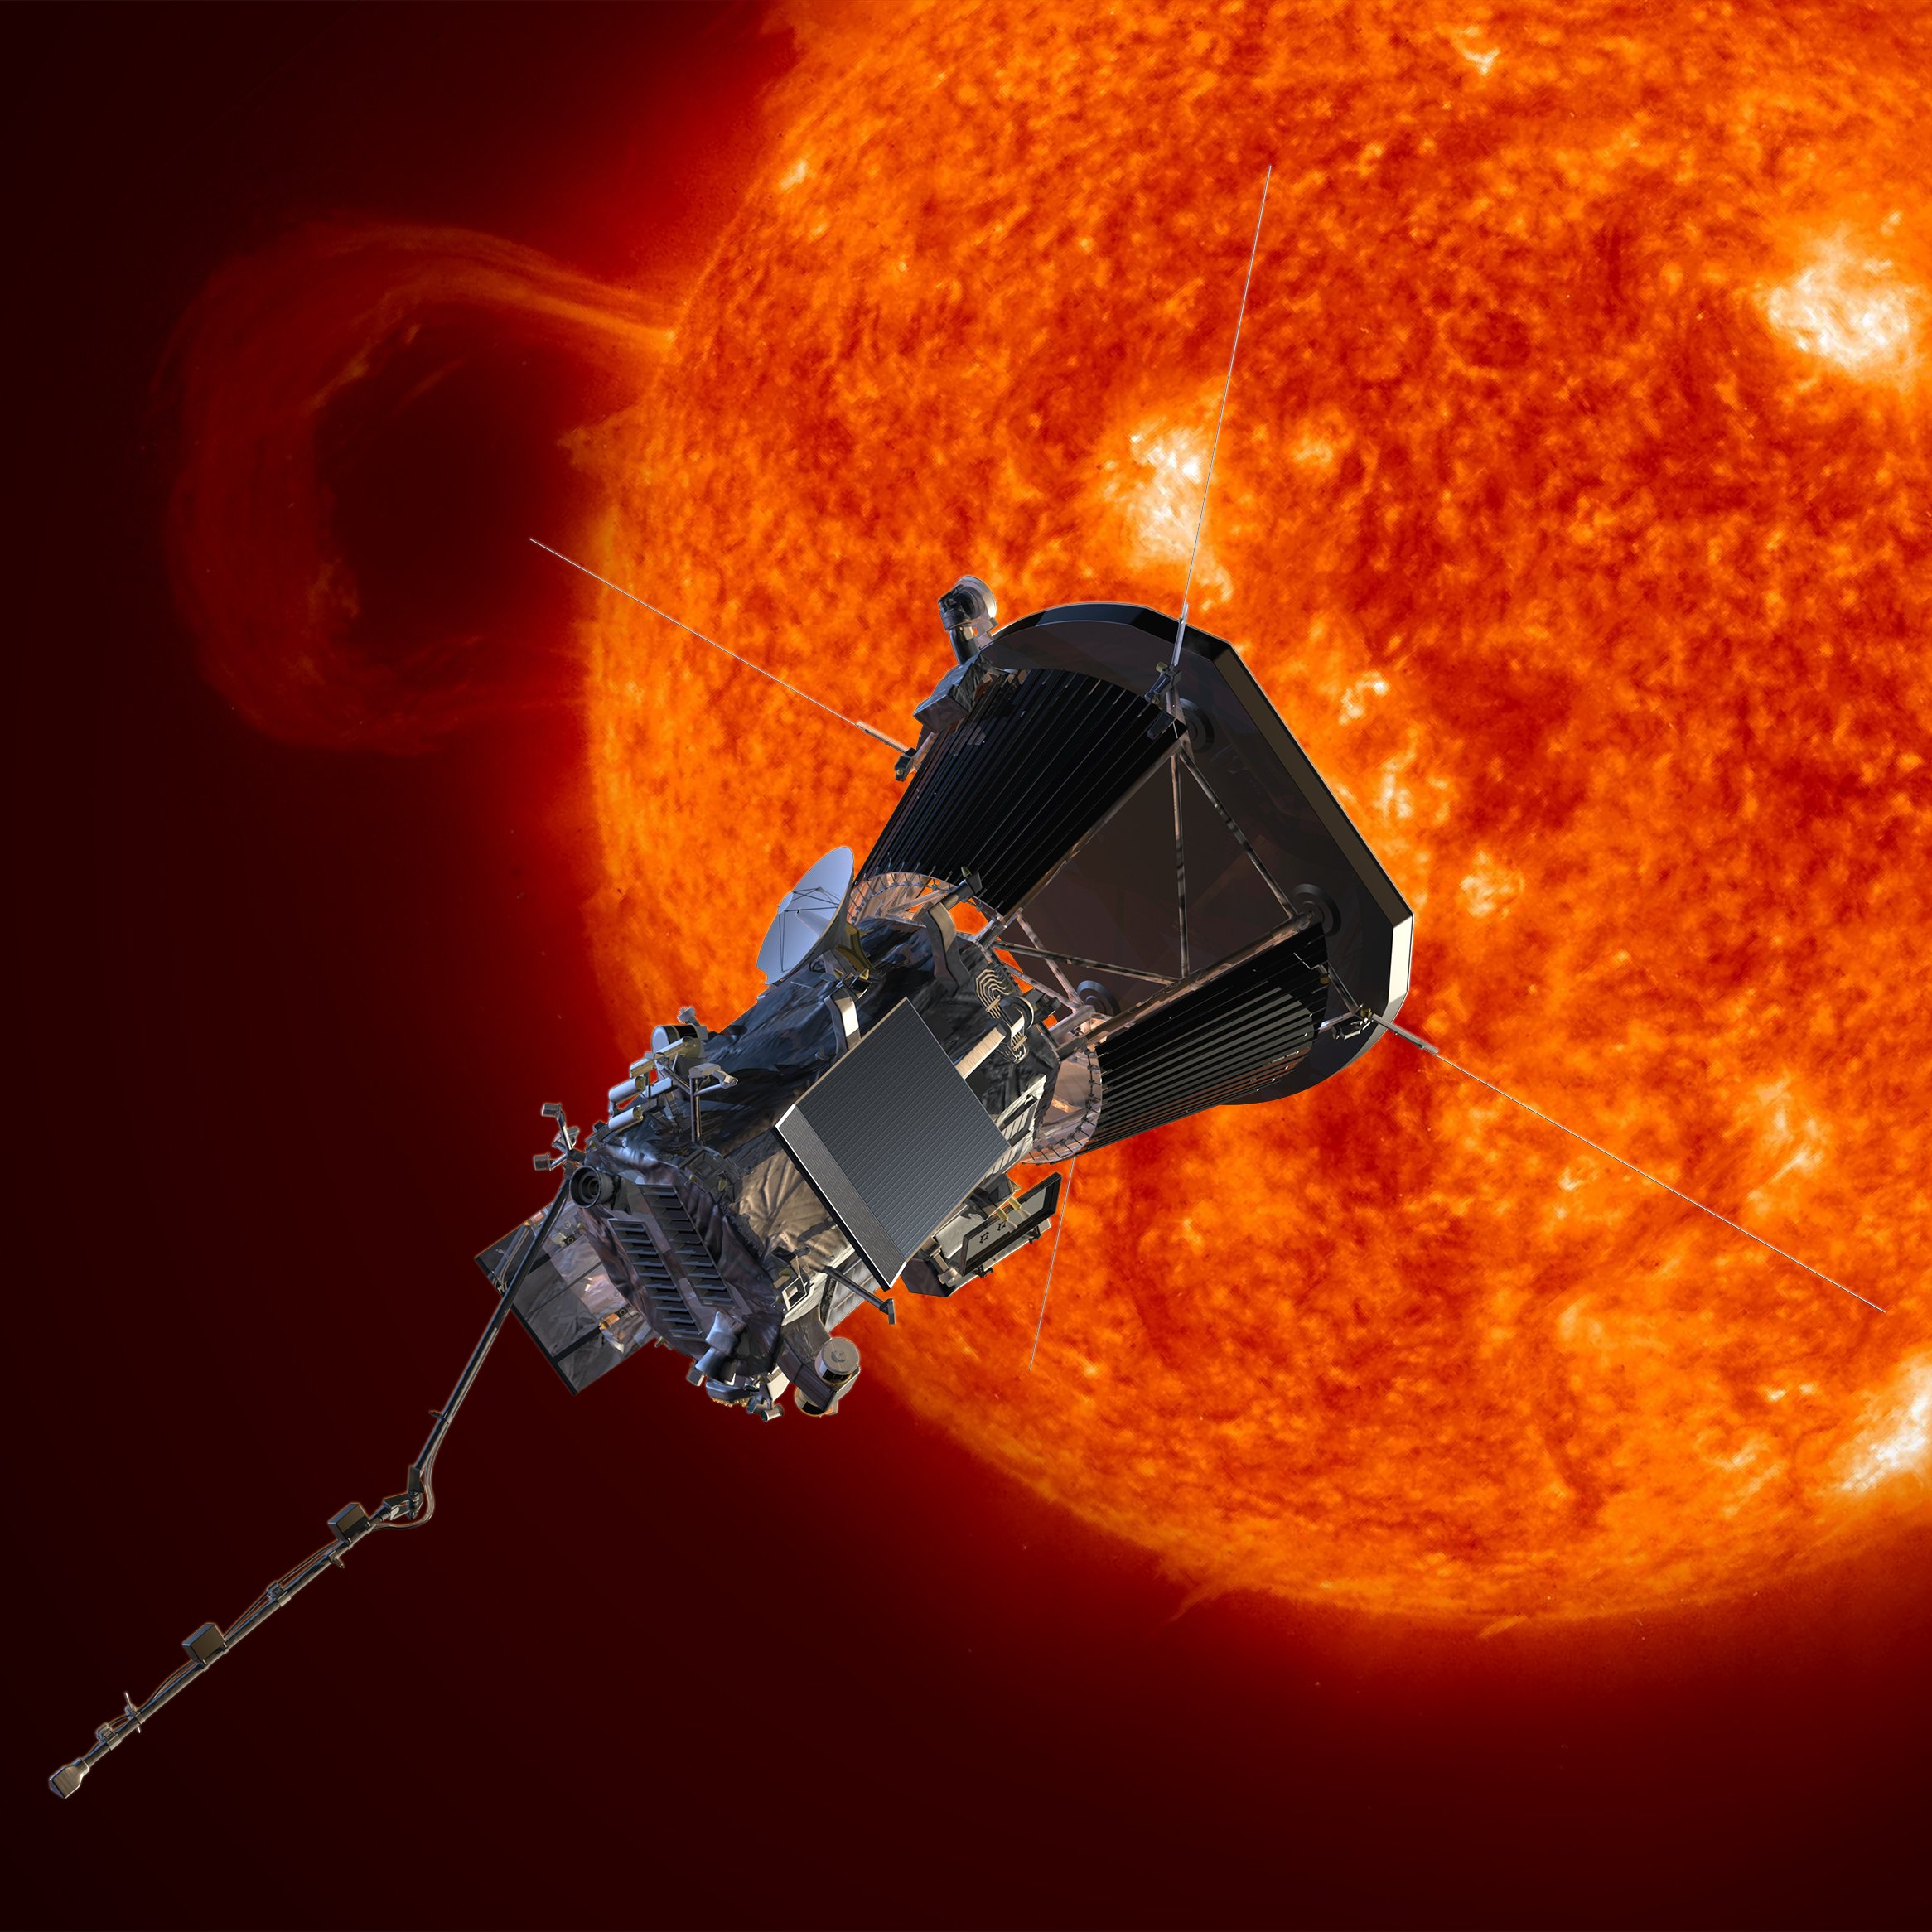
\includegraphics[width=0.46\textwidth]{figures_of_others/images/SPP_ObservingSun2_square.jpg}
		}{
			\caption[\lofimage{figures_of_others/images/SPP_ObservingSun2_square.jpg}Credit: \href{http://parkersolarprobe.jhuapl.edu/Multimedia/Images.php}{NASA/Johns Hopkins APL}, 2015.]
			{Artist’s concept of PSP near the Sun. Credit: \href{http://parkersolarprobe.jhuapl.edu/Multimedia/Images.php}{NASA/Johns Hopkins APL/Steve Gribben}, 2015.}
			\label{fig:SPP_ObservingSun2}
		}
		% http://parkersolarprobe.jhuapl.edu/Multimedia/ApprovedMedia/Images/Renderings/originals/SPP_ObservingSun2.jpg
		% http://parkersolarprobe.jhuapl.edu/Multimedia/Images.php
		%NASA has no copyrights to its contents (NASA FOIA)
		\ffigbox{
			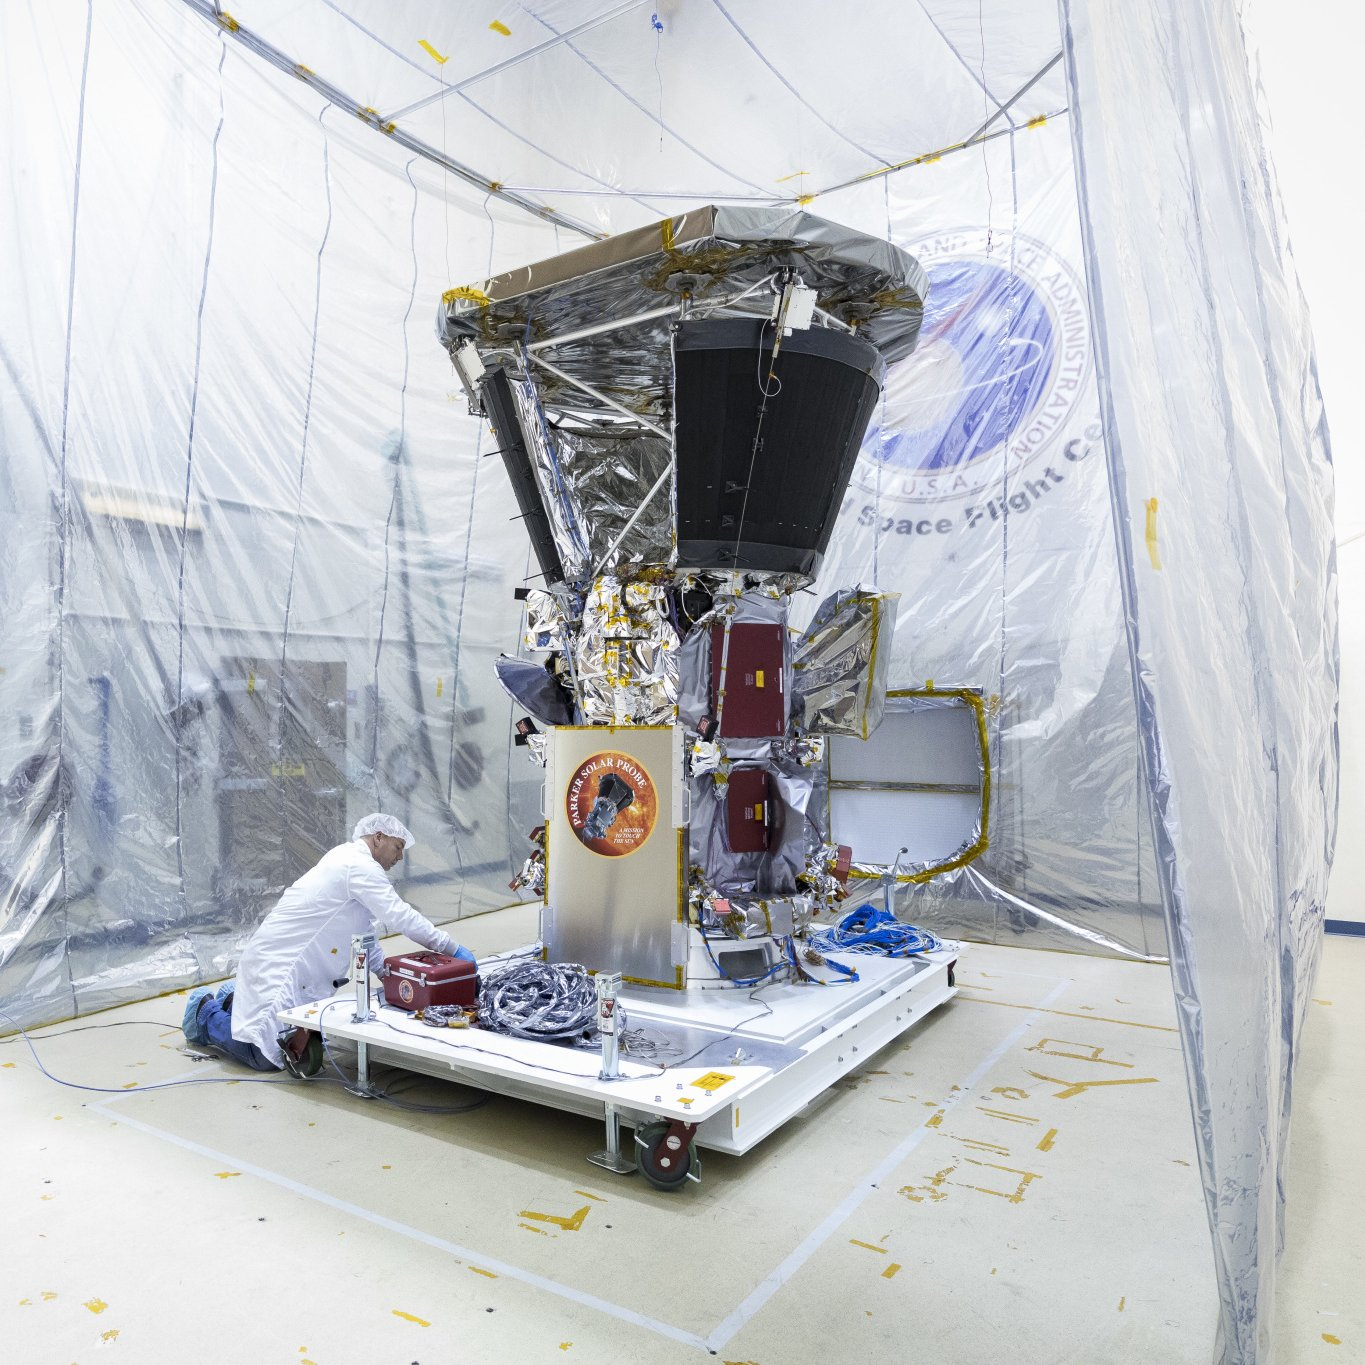
\includegraphics[width=0.46\textwidth]{figures_of_others/images/aa-roll-sc-into-acoustics-cell-0199_square.jpg}
		}{
			\caption[\lofimage{figures_of_others/images/aa-roll-sc-into-acoustics-cell-0199_square.jpg}Credit: \href{http://parkersolarprobe.jhuapl.edu/News-Center/Show-Article.php?articleID=62}{NASA/Johns Hopkins APL/Ed Whitman}, 2017.]
			{PSP in the Acoustic Test Chamber at NASA’s Goddard Space Flight Center in November 2017. Credit: \href{http://parkersolarprobe.jhuapl.edu/News-Center/Show-Article.php?articleID=62}{NASA/Johns Hopkins APL/Ed Whitman}, 2017.}
			\label{fig:aa-roll-sc-into-acoustics-cell-0199}
		}
		% http://parkersolarprobe.jhuapl.edu/News-Center/Show-Article.php?articleID=62
		% http://parkersolarprobe.jhuapl.edu/News-Center/admin/Press-Releases/images/articles/aa-roll-sc-into-acoustics-cell-0199.jpg
		%NASA has no copyrights to its contents (NASA FOIA)
	\end{floatrow}
\end{figure}
The large variations in solar power during the orbit, due to its high ellipticity, are addressed via changing the angle of the solar panels with solar distance. A photo of PSP during testing is shown in \autoref{fig:aa-roll-sc-into-acoustics-cell-0199}. As the communication is limited during the close encounters with the Sun, each orbit is splitted into a science operations and a data downlink phase. When the spacecraft is closer than \SI{0.25}{\au}, the scientific measurements are collected and when it is further away the data is downlinked.

There are four scientific experiments onboard PSP that contribute in redundant ways to the measurements of magnetic fields, plasma, waves, and SEPs \citep{Fox2015}.
The Electromagnetic Fields Investigation (FIELDS) consists of two fluxgate and one search coil magnetometer and five electric antennas \citep{Bale2016}. % measuring electric and magnetic fields and waves, spacecraft floating potential, density fluctuations, and radio emissions.
The Integrated Science Investigation of the Sun, Energetic Particle Instruments (IS\sun{}IS) has two instruments for different energy ranges, EPI-Hi and EPI-Lo \citep{McComas2016}. %This suite will make observations of energetic electrons, protons and heavy ions that are accelerated to high energies (10 s of keV to 100 MeV) in the Sun’s atmosphere and inner heliosphere.
The Solar Wind Electrons Alphas and Protons Investigation (SWEAP) is composed of two electrostatic analyzers and a Faraday cup \citep{Kasper2016}. %This investigation will count the most abundant particles in the solar wind—electrons, protons and helium ions—and measure their properties such as velocity, density, and temperature.
The Wide Field Imager for Solar Probe Plus (WISPR) is a white-light telescope for the solar corona and the inner heliosphere \citep{Vourlidas2016}. WISPR is to provide images of those solar wind structures PSP is about to fly through and measure in-situ. % This investigation complements the other instruments on the spacecraft providing direct measurements by imaging the plasma the other instruments sample.

The study in \citet{Venzmer2018} is conducted within the Coronagraphic German And US SolarProbePlus Survey (CGAUSS) which is the German contribution to the PSP mission as part of WISPR. The input of this study to the CGAUSS project is the extrapolation of Helios solar wind data to the solar distances PSP is to reach.


\section{On the published article}
%%% contributions and copyright
The major part of this chapter is published under the title ``Solar-wind predictions for the Parker Solar Probe orbit'' in \citet{Venzmer2018}, which is also just referred to as 'the paper' in this chapter. The article was published online on 20~March 2018 in Astronomy and Astrophysics (A\&A). It is included following this chapter, denoted as \autoref{chap:solar_wind_predictions_for_the_parker_solar_probe_orbit}. The European Southern Observatory (ESO) is the holder of the copyright -- the article is reproduced with permission.

The analyses presented in the paper were entirely done by myself, as well as the tables, figures, and equations. My coauthor Volker~Bothmer contributed significantly to the text and the anonymous referee helped clarifying a few aspects. The text was further improved by the A\&A language editor Joshua~Neve.
% my own contributions to the paper (percentages):\\
% data analyses 100\\
% tables 100\\
% figures 100\\
% formulas 100\\
% section structure 80\\
% text 55\\
% - abstract 70\\
% - introduction 30\\
% - frequency distributions 65\\
% - solar activity dependence 70\\
% - solar distance dependency 60\\
% - empirical solar wind model 75\\
% - model extrapolation 35\\
% - discussion and summary 20\\

The paper is included in \autoref{chap:solar_wind_predictions_for_the_parker_solar_probe_orbit}, so I will only briefly outline its content here: In the paper, we predict the solar wind conditions for the orbit of the PSP spacecraft. We extrapolate the near-Sun environment from empirical solar wind models that are based on Helios and OMNI solar wind observations. These estimations are further adjusted to the solar activity expected during the PSP mission -- the adjustments are based on empirical relations with the sunspot number (SSN).

% methods
The solar wind predictions are achieved via the following steps: We obtain lognormal representations of the frequency distributions’ shapes of the four key solar wind parameters magnetic field strength, proton velocity, density, and temperature. We derive analytical relations for the parameters’ solar activity dependencies and for their solar distance scaling. An empirical solar wind model is built from the combination of the obtained frequency distributions, SSN dependence relations, and solar distance dependence functions. The empirical model represents the solar wind’s solar activity and distance behavior, is fed with SSN predictions and extrapolated to the orbit of PSP.

We estimate the solar wind median values during PSP’s first perihelion and also model the values for PSP’s closest perihelia. The extrapolated values of the velocity and temperature lie above those obtained via remote observations in previous studies. This suggests that the region where the solar wind is accelerated and heated reaches up to distances of \SI{20}{\Rs} and thus will indeed be probed by the PSP spacecraft.

After the publishing of the paper, PSP's launch date was shifted from initially 31~July to 11~August 2018. This also shifts the date of the first perihelion by a few days to 5~November 2018, thus, the dates in Figure~12 of the paper have to be shifted by about seven days.

...does it shift the following perihelia as well??\\


\section{Parker magnetic field solar distance dependency}
% intro
In our article we noted that the model's near-Sun field magnitude, extrapolated to PSP's closest perihelion, will be lower than the actual values to be found. We scaled the magnetic field strength via a power-law function and obtained a solar-distance dependency proportional to $r^{-1.662}$. However, it is a simplified approach -- in the following I present a procedure, leading to an improved distance dependency, which is intended to account for the Parker IMF geometry, respecting the contributions of the individual field vector components, which have different power-law scalings. It is found that Voyager~1 observations of the magnetic field strength at solar distances larger than \SI{1}{\au} agree well with Parker’s IMF model \citep{Burlaga1984,Burlaga2002}.

The newly derived distance dependency, extrapolated to the PSP orbit and combined with the solar activity dependency described in the paper, yields \SI{8}{\%} higher values at the first perihelion and \SI{32}{\%} higher values at the closest perihelion in comparison to the estimates derived in the paper. In the following, this alternative distance dependency for the IMF model is derived. It is assumed to be more accurate for the near-Sun region.

\subsection{Parker magnetic field}
The coronal magnetic field near the Sun rotates rigidly, holding on to the coronal plasma. At the solar wind source surface, at around \SI{2.5}{\Rs} where the thermal plasma pressure overcomes the magnetic pressure, the magnetic field gets transported outwards in a radial way, maintaining only its radial vector component $\vect{B}_r$. From there on, the solar rotation begins to shear the magnetic field, building up a longitudinal component $\vect{B}_\phi$ as well. This solar wind magnetic field model was formulated by \citet{Parker1958} and has the following components in spherical coordinates ($\theta$ is the colatitude):
\begin{align}
	\vect{B}_r(r) &= B_0 \left(\frac{r_0}{r}\right)^2 \cdot \vect{e}_r\,,\\
	\vect{B}_\phi(r) &= -B_0 \left(\frac{r_0}{r}\right)^2 \cdot \frac{\omega\,r\,\sin\theta}{v_\text{sw}} \cdot \vect{e}_\phi	\,,	\label{eq:b_phi_vector}\\
	\vect{B}_\theta(r) &= 0 \cdot \vect{e}_\theta\,.
\end{align}
$B_0$ represents the radial field component at the solar distance $r_0$. The solar surface equatorial angular rotation rate $\omega$ and the solar wind velocity $v_\text{sw}$ are involved as well. From these equations it can be seen that $\vect{B}_r$ scales with increasing solar distance with $r^{-2}$, as it is expected for a spherical outflow, and $\vect{B}_\phi$ scales with $r^{-1}$ as expected for a two-dimensional point source. In-situ observations support the component's scaling according to these theoretical exponents, although in slow solar wind the scaling for $\vect{B}_\phi$ deviates somewhat from theory \citep{Mariani1978}.

From the magnetic field's absolute value
\begin{align}
	B(r) &= \sqrt{\vect{B}_r^2 + \vect{B}_\phi^2 + \vect{B}_\theta^2}\,,	\label{eq:B_absolute}\\
	B(r) &= \sqrt{\left(B_0 \left(\frac{r_0}{r}\right)^2\right)^2 + \left(-B_0 \left(\frac{r_0}{r}\right)^2 \cdot \frac{\omega\,r\,\sin\theta}{v_\text{sw}}\right)^2}\,,
\end{align}
it is apparent that the magnetic field strength does not scale with a simple power law. If the solar dipole axis tilt to the solar rotation axis is neglected and the radial field component $B_0$ is set to be in the equatorial plane at $r_0 = \SI{1}{\au}$, then $\theta = 90\degree$ and therefore
\begin{align}
	B(r) &= B_0 \cdot \sqrt{r^{-4} + \left(\frac{\omega\,r}{v_\text{sw}}\right)^2 r^{-4}}\,,	\label{eq:B_1au}
\end{align}
with the solar distance $r$ in astronomical units.

%%% field angle phi %%%
The magnetic field angle in the solar equatorial plane is distance dependent and is calculated via
\begin{align}
	\phi_B(r) &= \arctan\left(-\frac{\omega \cdot r}{v_\text{sw}}\right)	\,.	\label{eq:B_at_1au}
\end{align}
The angle becomes $\phi_B(\SI{1}{\au}) = \SI{-46.23}{\degree}$ when using the Sun's equatorial angular velocity $\omega_\text{eq} = \SI{14.37}{\degree\per\day}$ (for more details on solar rotation see Appendix~\ref{sec:solar_surface_differential_rotation}) together with the median solar wind velocity $v_\text{sw} = \SI{416}{\km\per\s}$ determined in the paper. During solar cycle minimum, the solar wind in the equatorial plane outside the source surface originates from polar regions at about \SI{+-60}{\degree} heliolatitude. This leads to a slightly underwound Parker spiral, because of the slower rotation rate at higher latitudes \citep{Banaszkiewicz1998}. Using the differential rotation rate $\omega(\SI{+-60}{\degree}) = \SI{13.69}{\degree\per\day}$ (see Appendix~\ref{eq:omega_differential}), the field angle becomes $\phi_B(\SI{1}{\au}) = \SI{-44.84}{\degree}$. As the solar rotation axis tilt to the ecliptic normal only has a maximum angle of \SI{7.2}{\degree}, I consider its influence on $\phi_B$ minor, and choose to neglect it in this calculation. Thus from theory, in the ecliptic at a solar distance of \SI{1}{\au}, the Parker spiral's observed magnetic field angle $\phi_B$ is centered most of the time at about \SI{-45}{\degree} or for the opposite field polarity at \SI{135}{\degree}. Indeed, this is confirmed by the angle's frequency distribution, apparent in IMF measurements made at \SI{1}{\au}, such as the OMNI data of the time period 1963--2016 plotted in \autoref{fig:histogram_B_angles_c}.
\begin{figure}[htb]
	\fcapside[\FBwidth]{
		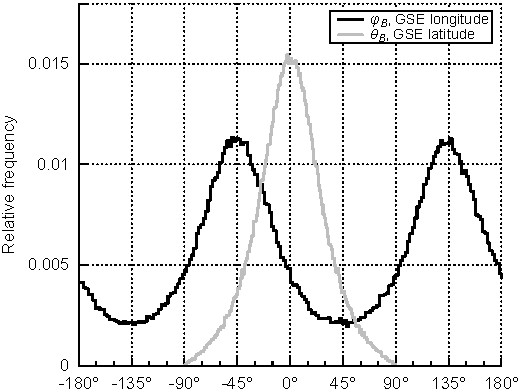
\includegraphics[width=0.6\textwidth]{figures_of_mine/gnuplots/histogram_B_angles_c.pdf}
	}{
		\caption{Frequency distributions of the magnetic field angles $\phi_B$ and $\theta_B$ in GSE coordinates. The frequencies are based on the hourly OMNI data during the period 1963--2016.}
		\label{fig:histogram_B_angles_c}
	}
\end{figure}

For $\phi_B$ being in average centered around these two directions, both vector components $\vect{B}_r$ and $\vect{B}_\phi$ have to be of equal amplitude. It can be seen from Equations~\ref{eq:B_absolute} and \ref{eq:B_1au} that this condition leads to
\begin{align}
	B(\SI{1}{\au}) &= B_0 \cdot \sqrt{2}	&\text{with}	&	&	\left(\frac{\omega\cdot\SI{1}{\au}}{v_\text{sw}}\right) &= 1\,.
\end{align}
Admittedly, this way $\omega$ and $v_\text{sw}$ are treated as time independent constants, which is a more valid approximation for $\omega$ than for $v_\text{sw}$.

\subsection{Solar distance dependency}
%%% fit %%%
Here, the magnetic field strength's distance dependency is derived in a similar way as in the paper \autoref{sec:paper_solar_distance_dependency}. Also, the same data set is used for the fitting process, that is, the combined in-situ data from the Helios~1 and Helios~2 spacecraft within the time range 1974--1981 (see also \autoref{sec:helios_probes}). The plain difference is the additional consideration of the longitudinal field component.

In order to get an analytical representation of the radial dependence of the magnetic field, I construct a suitable fit function based on \autoref{eq:B_at_1au}, assuming a nonexistent $\vect{B}_\theta$:
\begin{align}
	x(r) = a \cdot \sqrt{\left(r^{e_1}\right)^2 + \left(r^{e_2}\right)^2}	\,.	\label{eq:sqare_power_law}
\end{align}
The function, containing the scaling parameter $a$, and the exponents $e_1$ and $e_2$, is used in a least squares regression fit.

Within the Helios distance range \SIrange{0.3}{1.0}{\au}, the resulting fit curves are very similar to those in the paper -- as they are expected to be. The fit curves for the mean and median field strength are plotted with respect to solar distance in \autoref{fig:radial_fit_B_thesis_skip}. The graph is visually almost indistinguishable to the corresponding one in the paper Figure~7, \autoref{sec:paper_solar_distance_dependency}.
\begin{figure}[htb]
	\fcapside[\FBwidth]{
		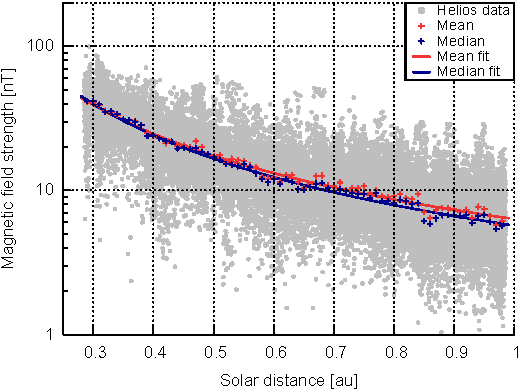
\includegraphics[width=0.6\textwidth]{figures_of_mine/gnuplots/radial_fit_B_thesis_skip.pdf}
	}{
		\caption{Magnetic field strength with respect to solar distance. The mean and median per \SI{0.01}{\au} data bin and their fit curves are plotted as well. The hourly Helios data has a native distance resolution of \SI{0.01}{\au}, thus, to make the distribution visible in this plot, I added a random distance value of up to \SI{+-0.005}{\au}.}
		\label{fig:radial_fit_B_thesis_skip}
	}
\end{figure}
The resulting curve fit parameters are presented in \autoref{tab:bfield_fit_parameters}.
\begin{table*}
	\caption{Fit coefficients for the curve fits (\autoref{eq:sqare_power_law}) and for the distribution fit (using the lognormal function of Equation~(4) from the paper), derived from the combined Helios~1 and 2 data. The numbers in parentheses are the errors on the corresponding last digits of the quoted value. The crossing distance indicates where the median and mean fits intersect each other. This distance is calculated numerically and its corresponding error only represents an estimated value.}
	\label{tab:bfield_fit_parameters}
	\centering
	\sisetup{table-figures-integer=1, table-figures-decimal=4, table-figures-exponent=0}
	\begin{tabular}{l l c c c c}
		\hline\hline
		\multirow{2}{*}{Fit}	&	&Factor	&\multicolumn{2}{c}{Exponents}	&Crossing distance\\
		\cline{4-5}
			&	&$a$	&$e_1$	&$e_2$	&[au]\\
		\hline
		\multirow{2}{*}{Curve}	&Median	&4.04(13)	&-1.852(25)	&-0.97(23)	&\multirow{2}{*}{0.336(10)}\\
			&Mean	&4.47(12)	&-1.740(18)	&-0.99(23)	&\\
		\multirow{2}{*}{Distribution}	&Median	&3.833(27)	&\multirow{2}{*}{-1.858(42)}	&\multirow{2}{*}{-1.32(12)}	&\multirow{2}{*}{--}\\
			&Mean	&4.081(29)	&	&	&\\
		\hline
	\end{tabular}
\end{table*}
%%% radial fit %%%
%4.47274*sqrt((r**-1.74028)**2 + (r**-0.990334)**2) = 4.04003*sqrt((r**-1.85224)**2 + (r**-0.974274)**2)\\
%r approx 0.336257719\\
%fit values
%4.04003	-1.85224	-0.974274
%4.47274	-1.74028	-0.990334
%errors
%0.130076	0.0246453	0.227053
%0.119049	0.0178415	0.228909
%table format
%4.04(13)	-1.852(25)	-0.97(23)
%4.47(12)	-1.740(18)	-0.99(23)
%avg WSSR = 27607.2	-6%
%med WSSR = 22254.7	-9%
%old avg WSSR = 29339.9	for simple power law function a*r^b
%old med WSSR = 24586.6
%
%%% fixed fit %%%
% 4.08078	-1.85771	-1.32237
% 3.83306	-1.85771	-1.32237
% errors:
% 0.0291872	0.042217	0.115887
% 0.0265236	0.042217	0.115887
% for table formatted:
% 4.081(29)	-1.858(42)	-1.32(12)
% 3.833(27)	-1.858(42)	-1.32(12)
% WSSR = 1.44202
% 1267.19055342511	this fit; is 33 % higher
% 950.841158464094	paper fit
%GUM statement
Concerning the error notation, I adhere to the parentheses notation documented in the ``Guide to the expression of uncertainty in measurement'' (GUM) published by \citet{GUM2008}, where the numbers in parentheses are the errors on the corresponding last digits of the quoted value.

The weighted sum of the squared residuals (WSSR) of this fit slighly improved in comparison to that of the simple power-law function $x(r) = d \cdot r^e$ used in \citet{Venzmer2018}: \SI{6}{\%} for the median and \SI{9}{\%} for the mean. However, the mean and median fit curves remain fairly similar and still cross each other at about the same distance as in the paper.

From the theoretical considerations sketched above, the expected fit parameter values are: \mbox{$a \approx B(\SI{1}{\au}) / \sqrt{2}$}, $e_1 \approx -2$, and $e_2 \approx -1$. The here obtained fit parameter values are closer to the theoretical values than those derived in the paper. The exponents $e_{1, \text{med}} = -1.852$ and $e_{1, \text{avg}} = -1.740$ are up to \SI{13}{\%} larger than the theoretical exponent for $e_1$ and lead to a less steep slope near the Sun. However, they are about \SI{12}{\%} smaller than the power-law exponents derived in the paper, which have values of \num{-1.655} and \num{-1.546} respectively.

It can be seen from \autoref{fig:sw_extrapolation_ssn_median_gt1au_g} that although the new fit curve is slightly curved, both fits are congruent in the Helios data range.
\begin{figure}[htb]
	\fcapside[\FBwidth]{
		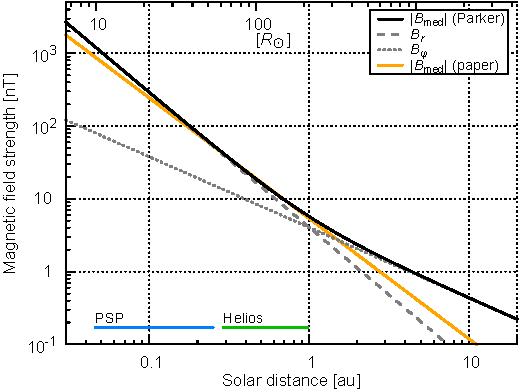
\includegraphics[width=0.6\textwidth]{figures_of_mine/gnuplots/sw_extrapolation_ssn_median_gt1au_g.pdf}
	}{
		\caption{Magnetic field strength fit curves with respect to solar distance. Plotted are the fitted absolute median field strength and its radial and azimuthal components. I added the absolute median field strength from Equation (10) of the paper as well. The orbital distance ranges from PSP and the Helios probes are indicated by the blue and green lines.}
		\label{fig:sw_extrapolation_ssn_median_gt1au_g}
	}
\end{figure}
But already little above \SI{1}{\au}, the power law yields significantly lower IMF strenghts. It is known that the decline in IMF strength behaves according to Parker's theory, at least in the range \SIrange{1}{81}{\au} \citep{Burlaga2002}. However, both curves deviate less pronounced in the PSP distance range \SIrange{0.046}{0.25}{\au}.

In the next step, a lognormal function is fitted to the data -- I use the same method and reasoning as explained in the paper's \autoref{sec:paper_solar_distance_dependency}. Therefore the IMF distribution's shapes are considered to be lognormal at all distances and the fit exponents $e_\text{med}$ and $e_\text{avg}$ are reduced to only one common exponent. The distance dependency is implemented into the lognormal function from the paper, yielding in the parameters and common exponents of the distribution fit. The fit parameters are presented in \autoref{tab:bfield_fit_parameters} and the fitted distribution is plotted in \autoref{fig:fit_fixed_B_paper_f}.
\begin{figure}[htb]
	\fcapside[\FBwidth]{
		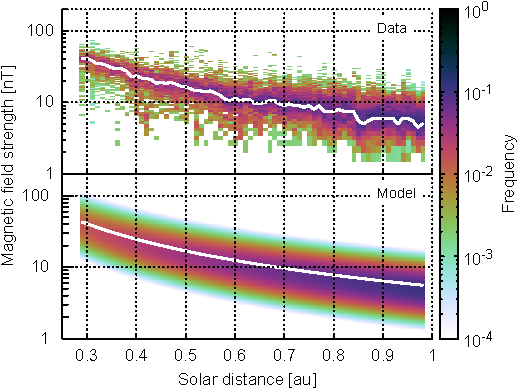
\includegraphics[width=0.6\textwidth]{figures_of_mine/gnuplots/fit_fixed_B_paper_f.pdf}
	}{
		\caption{Frequency distribution of the solar wind magnetic field strength with respect to solar distance. I plotted the binned Helios data (top panel) and the square-root power-law lognormal fit model (bottom panel) with their median values (white lines).}
		\label{fig:fit_fixed_B_paper_f}
	}
\end{figure}
The fitted distribution looks almost identical to the corresponding one presented in Figure~8 of the paper. This is expected -- it is the same aspect as for \autoref{fig:radial_fit_B_thesis_skip}.

\subsection{SSN implementation and extrapolation to PSP orbit}
Finally, the IMF distance dependency will be combined with the solar activity relationship obtained in the paper. In order to derive the solar wind environment for the PSP orbit, the model is then extrapolated to the PSP orbit.

To take into account predictions of the SSN, the distance relation is used to scale the SSN-relation for \SI{1}{\au}:
\begin{align}
	B(ssn,r) = \frac{B(ssn)}{\sqrt{2}} \cdot \sqrt{\left(r^{e_1}\right)^2 + \left(r^{e_2}\right)^2}	\,.
\end{align}
This way the square root just replaces the $r^{-1.66}$ factor of Equation~(12) in the paper:
\begin{align}
	B_\text{med}(ssn,r) &= \left(\SI{0.0131}{\nT} \cdot ssn + \SI{4.29}{\nT}\right) \cdot \sqrt{\left(r^{-1.86}\right)^2 + \left(r^{-1.3}\right)^2}	\,.
\end{align}

This magnetic field strength model can now be extrapolated to PSP's orbital range. \autoref{fig:sw_extrapolation_ssn_g} shows the model and its extrapolation, visualized for a SSN range \numrange{0}{200}, representing the range from solar minimum to maximum. The magnetic field strength from the paper is shaded in yellow, the above derived model in the Helios range in green and its extrapolation to the PSP range in blue. The newly derived model is found to differ increasingly going closer to the perihelion of the extrapolated PSP region.
\begin{figure}[htb]
	\fcapside[\FBwidth]{
		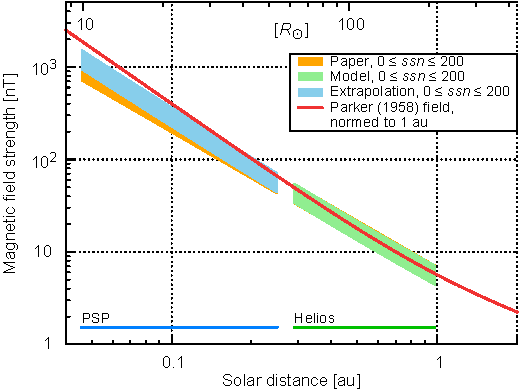
\includegraphics[width=0.6\textwidth]{figures_of_mine/gnuplots/sw_extrapolation_ssn_g.pdf}
	}{
		\caption{Radial extrapolation of the solar wind magnetic field strength to the PSP orbit region. The median value from the model, obtained from Helios and OMNI measurements, is extrapolated to the PSP region for SSN values between solar minimum and maximum, that is, $0 \le ssn \le 200$. The lower edges of the shaded areas correspond to solar minimum, the upper edges to solar maximum. I also added the model from the paper (yellow) and the radial dependency of the field model by \citet{Parker1958}, normed to \SI{1}{\au} (red). The orbital distance ranges from PSP and the Helios probes are indicated by the blue and green lines.}
		\label{fig:sw_extrapolation_ssn_g}
	}
\end{figure}

The \citet{Parker1958} field model with the theoretical exponents, normed to \SI{1}{\au}, is drawn for comparison. It features an even larger curvature than the derived model which exhibits exponents adjusted by the fit to the Helios data.

The solar wind environment can be forecasted to PSP's orbit and mission time, using the same SSN predictions as described in the paper, that is, the SIDC forecast and mirroring of the last solar cycle. The magnetic field changes during the first perihelion and the first closest perihelion (which is actually the 22nd) are plotted in \autoref{fig:PSP_perihelia_prediction_f}.
\begin{figure}[htb]
	\fcapside[\FBwidth]{
		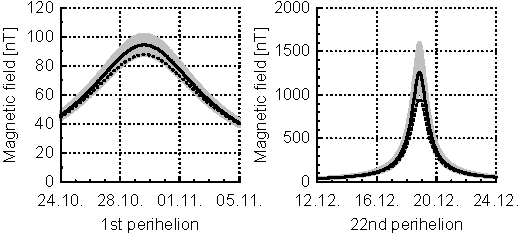
\includegraphics[width=0.6\textwidth]{figures_of_mine/gnuplots/PSP_perihelia_prediction_f.pdf}
	}{
		\caption{Estimated magnetic field strength medians (solid lines) and their error bands (gray area) during 12~days in 2018 and 2024 with PSP's first perihelion at about \SI{0.16}{\au} and PSP's 22nd perihelion at \SI{0.046}{\au}. I indicated the prediction from \citet{Venzmer2018} as well (dotted lines).}
		\label{fig:PSP_perihelia_prediction_f}
	}
\end{figure}
% first perihelion value:
% 94 nT	this fit; is 8 % higher
% 87 nT	old fit
% first closest perihelion value:
% 1241 nT	this fit; is 32 % higher
% 943 nT	old fit
The estimated magnetic field strength median value for PSP's first perihelion is with of \SI{94}{\nano\tesla} \SI{8}{\%} higher than that derived in the paper. The median value for the first closest perihelion is with \SI{1241}{\nano\tesla} even \SI{32}{\%} higher.

The model assumes a frequency distribution of lognormal shape and shifts this distribution according to solar activity and solar distance. The estimated IMF frequency distributions at \SI{1}{\au}, at PSP's first perihelion, and at its first closest perihelion are plotted in \autoref{fig:PSP_sw_distributions_c}.
\begin{figure}[htb]
	\fcapside[\FBwidth]{
		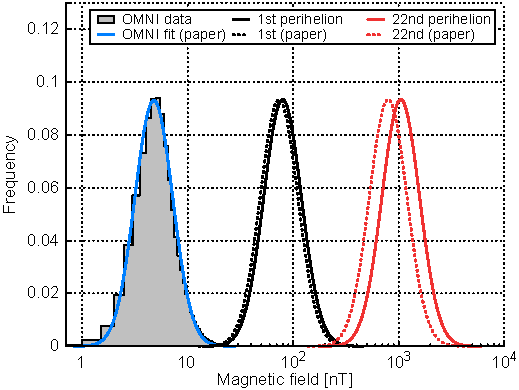
\includegraphics[width=0.6\textwidth]{figures_of_mine/gnuplots/PSP_sw_distributions_c.pdf}
	}{
		\caption{Frequency distribution of the magnetic field strength at \SI{1}{\au} (OMNI data and fit) and those estimated with the derived model for PSP's 1st and 22nd perihelion. In this plot the frequencies of both extrapolated curves are scaled up for visibility to the same peak frequency as the \SI{1}{\au} distribution. I indicated the predictions from \citet{Venzmer2018} as well (dotted lines).}
		\label{fig:PSP_sw_distributions_c}
	}
\end{figure}
It is evident that during the closest perihelion, strong magnetic fields are estimated to occur much more frequent than predicted from the model in the paper.

\subsection{Discussion}
The only difference between the magnetic field strength models presented in this section and in the paper lies in their differing solar distance relations. The models both still assume a lognormal distributed magnetic field strength and the same dependency on solar activity. Instead of being based on a simple power law, the solar distance relation derived above is based on the well-founded spiral field model formulated by \citet{Parker1958}. This newly derived IMF relation fits the Helios data as good as that one presented in \citet{Venzmer2018}. However, the function is slightly more curved so that the magnetic field becomes larger outside the fitted solar distance range \SIrange{0.3}{1}{\au}. The consequence is a significant increase in the predicted field strength at the perihelia of PSP's orbital trajectory, ranging from \SI{8}{\%} at the first perihelion to \SI{32}{\%} at the first closest perihelion.

% % % former outlook
Seasonal effects from the orbit of the Earth have an influence on the OMNI data set, as it represents measurements located at the bow shock of the magnetosphere. These effects include the Earth's solar distance and its heliographic latitude. It would be valuable to estimate how large the resulting errors for the models are.


\section{Possible solar wind model refinements}
Currently, the solar wind models described in the paper and in this chapter are purely empirical and the four solar wind quantities are characterized independently from each other. In further steps, theoretical relations connecting the parameters could be introduced to make the model more self-consistent. For example, proton flux conservation could be implemented into the radial distance dependencies, relating the two parameters density and velocity. Or also, the solar wind velocity within the magnetic field's azimuthal component (\autoref{eq:b_phi_vector}) could be respected as a variable and not as a constant as it is done in the previous section, relating the two parameters velocity and magnetic field strength.\\

see notes...\\


list principal conclusions of this study:\\
- \\


% There exist a lot more aspects related to solar wind that are not covered in this study, i.e., MHD waves, the electron pitch angle, solar energetic particles, dust particles, and neutral energetic atoms. It would be worth looking into these properties as well...\\

\bigskip
{\small
\textit{Acknowledgments.} Part of the research leading to the results presented in this chapter recieved support of the CGAUSS project for WISPR by the DLR under grant 50~OL~1601 as national contribution to the PSP mission.
The analyses in this chapter are based on the Helios and the OMNI data, which are supplied by the SPDF at GSFC (NASA). The author thanks the Helios and OMNI PIs/teams for creating and making available the solar wind in-situ data. Additional thank for maintaining and providing the international sunspot number series goes to the WDC-SILSO at the SIDC (ROB).
}

\section{notes...}
Schwenn1983 intro -> sw-averaging comment (beer and wine) (cite him...)\\
see Hellinger2013 p.1353\\
see Balogh1999 from p. 162 (Helios CIR results)\\

at larger distances (specify...) heating outbalances the adiabatic temperature part (adiabatic cooling vs. pickup proton and stream--interaction heating; 1--68~au by Voyager~2; \citet{Richardson2003}\\
solar wind ram pressure $p_\text{ram} = \rho V^2$\\

\subsection{flux conservation}
conserved quantities:\\
- momentum conservation... VBbookp112\\
- flux conservation...\\

%%%%%%%%%%%--  flux  --%%%%%%%%%%%%%%%
%As Schwenn1983 stated ``From Helios in situ measurements we know that at least beyond 0.29~au there is almost no nonradial flow, on the average. In fact, the particle flux was found to be that quantity which varies the least with increasing R.''\\

%Schwenn1990:
%increase in sw velocity with distance; speed increase mainly in slow solar wind
%density deviates from a purely r^-2 fall-off (10% faster); n(r)=6.1*r^-2.1 cm^-3; different behavior in slow and fast wind
%proton flux density constant between 0.3-1.0~au -> no meridional flow into/out of the ecliptic; different for slow and fast sw

With consideration of continuity, the mass flux per solid angle has to be constant: $\dot{m} = \text{const}$\\
conserved quantities:\\
- mass flux: $\dot{m} = \rho v A$ (with mass density $\rho$, velocity $v$ and solid angle A)\\
- particle fluxes (proton flux, electron flux, etc.)\\
	- proton flux: $j_\text{p} = n_\text{p} v_\text{p} A$ (with proton density $n_\text{p}$ and proton velocity $v_\text{p}$)\\

(with proton mass density $\rho = n_\text{p} m_\text{p}$ (with proton number density $n_\text{p}$ and proton mass $m_\text{p}$).)\\

the individual radial dependencies for a spherical radial outflow are:\\
$A(r) \propto r^2$ --> $A/r^2 = \text{const}$\\
and assuming exponential dependencies,\\
$n_{\text{p}}(r) = n_0 r^{c_n}$,\\
$v(r) = v_0 r^{c_v}$\\
\begin{align}
	j_\text{p} &= \text{const}\\
	n_\text{p} v_\text{p} A &= \text{const}\\
	n_0 r^{c_n} v_0 r^{c_v} r^2 &= \text{const}\\
	r^{c_n} r^{c_v} r^2 &= \text{const}\\
	\Rightarrow c_n + c_v + 2 &= 0\\
	c_n + c_v &= -2
\end{align}
Thus, an increasing velocity results in a steeper density fall-off.\\

validity of mass flux continuity: within the heliosphere mass to energy conversion and vice versa is negligible, but there can be flux from and to higher latitudes as the Helios data is localized to a small latitude range in the ecliptic plane.\\
larger errors should be located near CMEs and CIRs (nonradial flows from deflections)\\
there is a proton flux difference between slow and fast solar wind streams (see book Schwenn1990 p.~146)

estimate the possible size of error:\\
(constant mass flux only for mean)\\
$c_n = -2.114$\\
$c_v = 0.0990$\\
$c_n + c_v = -2.024$\\
difference to -2 is 0.024\\

simple view: For a spherical constant velocity mass outflow, a per distance squared law is expected for the density, because of the mass flux conservation per solid angle for different distances. Measurements up to the outer heliosphere confirm the $r^{-2}$ dependency (1--38~au by Voyager~2, \citep{Belcher1993} newer paper?)\\


\subsection{Seasonal solar wind variations}
seasonal variation by month\\
quantify variation amplitudes\\

see \autoref{fig:OMNI_monthly_freq_V_gps} and \autoref{fig:OMNI_monthly_freq_B_a_gps}\\
\begin{figure}[htb]
	\centering
	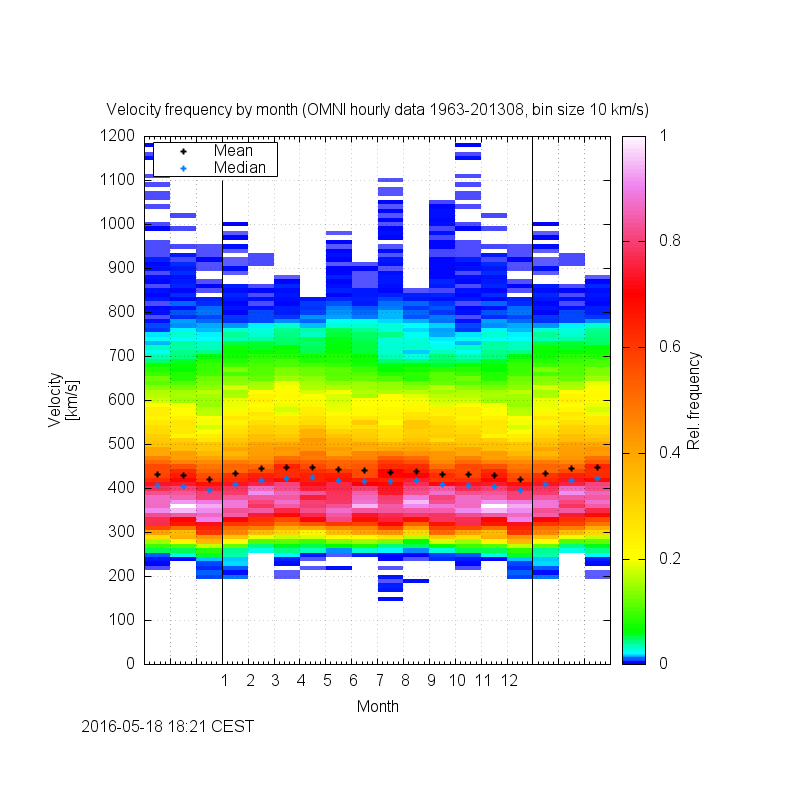
\includegraphics[width=0.3\textwidth]{figures_of_mine/gnuplots/OMNI_monthly_freq_V_gps.png}
	\caption{Diagram of the velocity frequency by month for the period 1963/01--2013/08. Mean and median values are shown as well.}
	\label{fig:OMNI_monthly_freq_V_gps}
\end{figure}
\begin{figure}[htb]
	\centering
	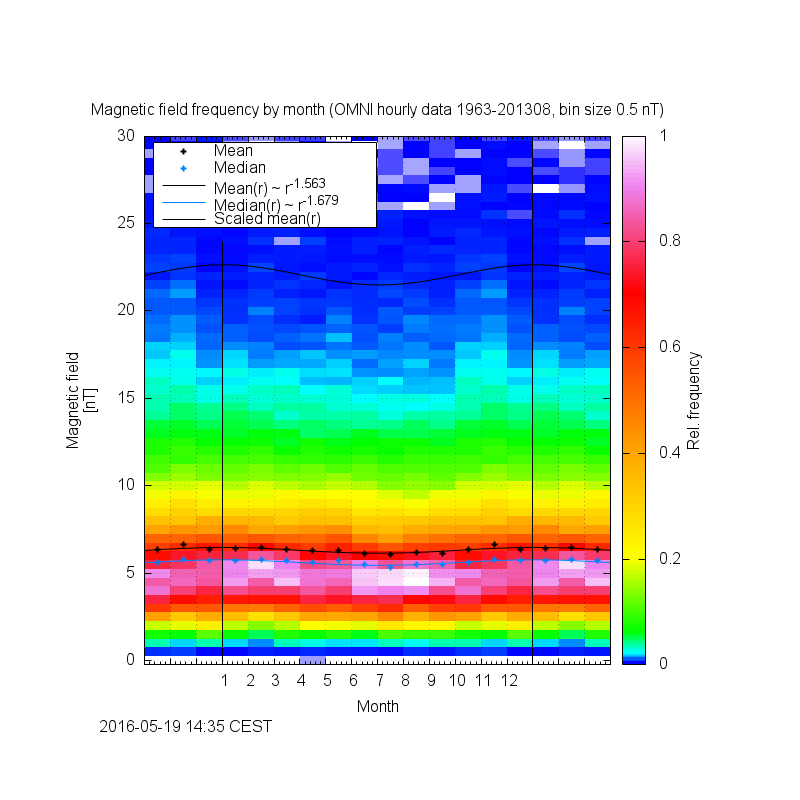
\includegraphics[width=0.3\textwidth]{figures_of_mine/gnuplots/OMNI_monthly_freq_B_a_gps.png}
	\caption{Diagram of magnetic field frequency by month for the period 1963/01--2013/08. Mean and median values are shown as well as the expected course from the solar distance variation (obtained from Helios data).}
	\label{fig:OMNI_monthly_freq_B_a_gps}
\end{figure}
make 4-panel figure...\\

derived exponent values from simple trigonometric fit on monthly values:\\
$c_n = -2.234$\\
maybe figure?\\

expected influence from Earth's perihelion/aphelion (see Appendix...) distance vs observations\\
we expect for the mean proton density (scaling law $n(r) \propto r^{-2.114}$):\\
$n(0.983~au) = 7.098~cm^{-3}$\\
$n(1~au) = 6.845~cm^{-3}$\\
$n(1.017~au) = 6.605~cm^{-3}$\\
we expect for the magnetic field strength (paper scaling law $n(r) \propto r^{-1.662}$):\\
$B(0.983~au) = 5.870~nT$\\
$B(1~au) = 5.705~nT$\\
$B(1.017~au) = 5.547~nT$\\


\subsection{Latitude dependency}
refer to Ulysses \autoref{fig:McComas2008_Ulysses_orbit}\\
Ulysses swoops polar plots...\\

see Schwenn1990's~Fig.~3.14\\
see also \citet{Schwenn1990} p.~127\\
see also \citet{Richardson1995}\\
Balogh et al. (1999) p. 162 ff (origin and formation of CIRs in inner heliosphere with Helios data; latitude V dependence)\\

Helios latitude; see \autoref{fig:latitude_frequency_4_thesis_plot}
\begin{figure}[htb]
	\centering
	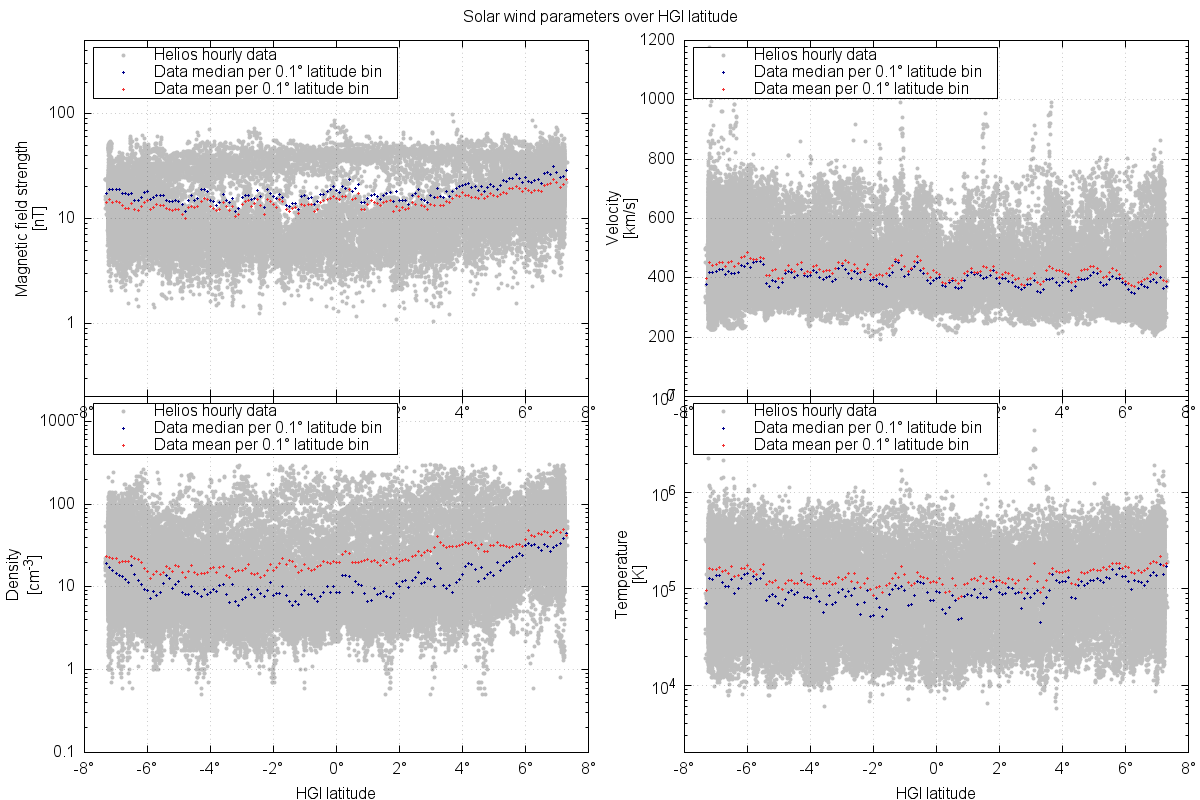
\includegraphics[width=0.5\textwidth]{figures_of_mine/gnuplots/latitude_frequency_4_thesis_plot.png}
	\caption{The four solar wind parameter's HGI latitude dependency. Their mean and median values per \SI{0.1}{\degree} bin are plotted as well. I added a random distance value of up to \SI{+-0.005}{\au} in order to make the distribution visible in this plot.}
	\label{fig:latitude_frequency_4_thesis_plot}
\end{figure}

with the exponential dependencies to 1~au projected solar wind parameters; there are only small changes with latitude in the range \SIrange{-7.25}{7.25}{\degree}\\
have a look on distribution widths...\\

dependence from latitude in interval \SIrange{-7.25}{7.25}{\degree} in Helios data negligible?, see \autoref{fig:latitude_frequency_rcorrected_v3_4_thesis_plot}.\\
\begin{figure}[htb]
	\centering
	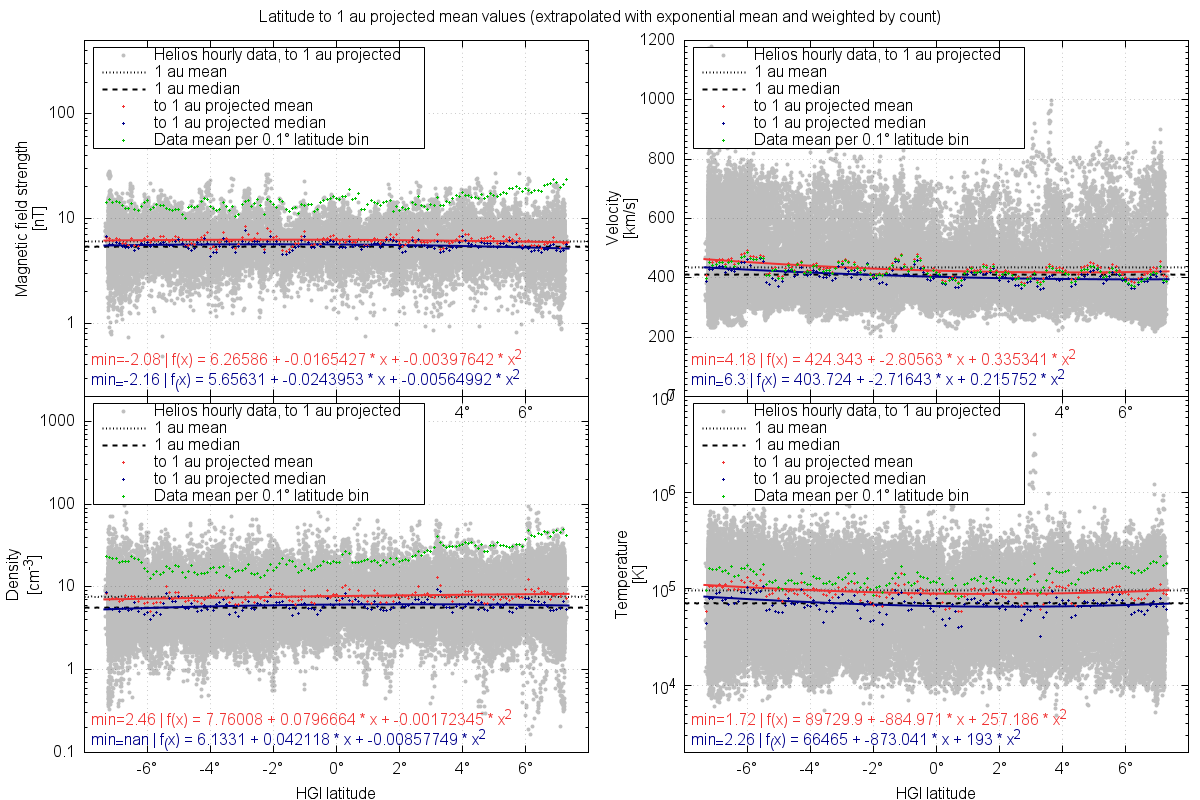
\includegraphics[width=0.5\textwidth]{figures_of_mine/gnuplots/latitude_frequency_rcorrected_v3_4_thesis_plot.png}
	\caption{Solar wind parameters projected to 1~au with respect to latitude. And their mean values, including weighted fit. I added a random distance value of up to \SI{+-0.005}{\au} in order to make the distribution visible in this plot. add projected median...}
	\label{fig:latitude_frequency_rcorrected_v3_4_thesis_plot}
\end{figure}
estimate error ranges from latitude influence...\\

...plot Ulysses data into plot?\\

%latitude variation negligible?
influence from latitude variation in data negligible? (see Ulysses \autoref{fig:McComas2008_Ulysses_orbit} in introduction). Helios probes within ecliptic => variation span equal to solar tilt: \SIrange{-7.25}{7.25}{\degree}; solar tilt/obliquity to ecliptic: $i_\odot = 7.25\degree$ (Sun fact sheet: \url{http://nssdc.gsfc.nasa.gov/planetary/factsheet/sunfact.html)}\\
big part of Helios data is from latitudes $>\pm5$°, see Figure~XX (data count over latitude) and see \autoref{fig:Helios12_orbits_ecliptic_polar} (Helios orbit polar plane in data section)\\

The Helios magnetic field and plasma data frequency over heliocentric distance and over heliographic latitude are plotted in \autoref{fig:helios_data_frequency}.\\
\begin{figure}[htb]
	\centering
	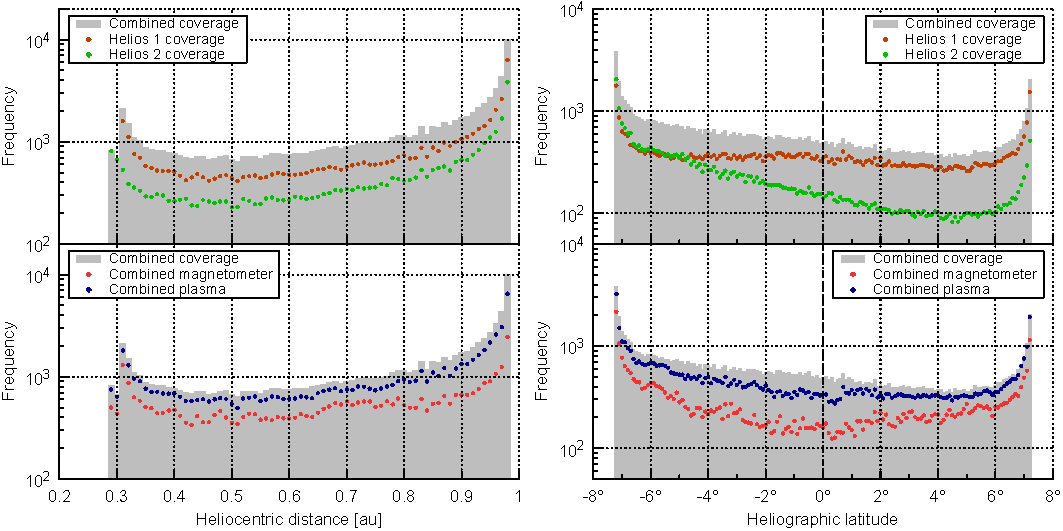
\includegraphics[width=\textwidth]{figures_of_mine/gnuplots/helios_data_frequency.pdf}
	\caption[\lofimage{figures_of_mine/gnuplots/helios_data_frequency.pdf}]
	{Helios data frequency over heliocentric distance with bins of \SI{0.01}{au} (left panels) and over heliographic latitude with bins of \SI{0.1}{\degree} (right panels). The frequency data is based on the hourly merged magnetometer and plasma data sets for Helios~1 and Helios~2. The top panels show the frequencies for Helios~1 and Helios~2 individually and the bottom panels those for the magnetometer and plasma data.}
	\label{fig:helios_data_frequency}
	\addtocontents{lof}{\smallskip\protect\center I created the figure myself.\medskip}
\end{figure}


\subsection{Radial evolution of solar wind structures}
see CGAUSS \url{report2015_2}

Helios event lists HSSs, SLOWs, CIRs, CMEs...; event lists for all Helios data\\
see Liu2004 for Helios ICME list and radial dependencies of $B$, $n$, $T$ and $v$...\\

\SI{200}{\km\per\s} slow solar wind at \SI{10}{\Rs} is in agreement with blob measurements from Wang2000\\

very slow sw (VSSW) gets accelerated; see Sanchez-Diaz2016:\\
%"The reported in situ measurements suggest that the properties of VSSW are a continuation of the slow wind toward lower speeds: higher densities, higher proton fluxes, and lower temperatures, thereby extending well-known scaling laws [Lopez and Freeman, 1986; Hundhausen et al., 1970] down to speeds as low as 200 km/s."\\
%"The VSSW has a number of interesting properties that suggest it may be the interplanetary signature of long HPS crossings."\\


radial diameter of MCs increase between 0.3~au and 4.3~au proportional to the distance as $r^{0.8}$ \citep{Bothmer1998}\\
MC central axial magnetic field strength radial density dependence $B = 18.1\,r^{-1.64}$ \citet{Leitner2007}\\
MC average diameter $D = 0.23\,r^{1.14}$ \citet{Leitner2007}

sw structure marked plots\\



\cleardoublepage
